\documentclass[UTF8,AutoFakeBold,AutoFakeSlant,zihao=-4]{ctexart}
\usepackage[a4paper,left=2.4cm,right=2.4cm,top=2.6cm,bottom=2.38cm,includeheadfoot]{geometry}   % 设置页面大小
\usepackage{fontspec} % 字体
\usepackage{setspace} % 设置行距
\usepackage{graphicx} % 图片
\usepackage{fancyhdr} % 页眉页脚
\usepackage{pdfpages} % 插入 PDF
\usepackage{setspace} % 设置行距
\usepackage{booktabs} % 表格
\usepackage{multirow} % 表格
\usepackage{caption} % 图片和表格的 caption
\usepackage{subcaption} 
\usepackage{float} 
\usepackage{listings}
\usepackage{color}
\usepackage[colorlinks,linkcolor=blue]{hyperref}

\definecolor{dkgreen}{rgb}{0,0.6,0}
\definecolor{gray}{rgb}{0.5,0.5,0.5}
\definecolor{mauve}{rgb}{0.58,0,0.82}

\lstset{frame=tb,
  language=Python,
  aboveskip=3mm,
  belowskip=3mm,
  showstringspaces=false,
  columns=flexible,
  basicstyle={\small\ttfamily},
  numbers=none,
  numberstyle=\tiny\color{gray},
  keywordstyle=\color{blue},
  commentstyle=\color{dkgreen},
  stringstyle=\color{mauve},
  breaklines=true,
  breakatwhitespace=true,
  tabsize=3
}


\newcommand{\coursename}{《Python程序设计》}
\newcommand{\coursenumber}{U08M11077.01}
\newcommand{\proname}{目标检测实例的复现}
\newcommand{\members}{敖冠舒~唐中磊~王骏松~王一帆}
\newcommand{\phone}{134~0324~7575}
\newcommand{\protime}{2022年12月}

% 定义 caption 字体为楷体
\DeclareCaptionFont{kaiticaption}{\kaishu \normalsize}

% 设置图片的 caption 格式
\renewcommand{\thefigure}{\thesection-\arabic{figure}}
\captionsetup[figure]{font=small,labelsep=space,skip=10bp,labelfont=bf,font=kaiticaption}

% 设置表格的 caption 格式
\renewcommand{\thetable}{\thesection-\arabic{table}}
\captionsetup[table]{font=small,labelsep=space,skip=10bp,labelfont=bf,font=kaiticaption}

% 定义一个概念
\newtheorem{definition}{概念}[section]

% 输出大写数字日期
\CTEXoptions[today=big]


\setromanfont{Times New Roman}



% 设置文档标题深度
\setcounter{tocdepth}{3}
\setcounter{secnumdepth}{3}

%%
% 设置一级标题、二级标题格式
% 一级标题:小三,宋体,加粗,段前段后各半行
\ctexset{section={
  format={\raggedright \bfseries \songti \zihao{-3}},
  beforeskip = 24bp plus 1ex minus .2ex,
  afterskip = 24bp plus .2ex,
  fixskip = true,
  name = {,.}
  }
}
% 二级标题:小四,宋体,加粗,段前段后各半行
\ctexset{subsection={
  format = {\bfseries \songti \raggedright \zihao{4}},
  beforeskip =24bp plus 1ex minus .2ex,
  afterskip = 24bp plus .2ex,
  fixskip = true,
  }
}

%%
% 文档开始
\begin{document}

% 报告封面
\topskip=0pt

\begin{titlepage}
  \vspace*{20mm}
  \centering
  \hspace{0mm}\heiti\fontsize{30pt}{30pt}\selectfont{西北工业大学}

  \vspace{13mm}

  \hspace{0mm}\heiti\fontsize{20pt}{20pt}\selectfont{课程设计(大作业)报告}

  \vspace{40mm}

  \flushleft
  \begin{spacing}{2.2}


    \hspace{36mm}\songti\fontsize{16pt}{16pt}\selectfont{\textbf{课程名称:}\underline{\makebox[72mm][c]{\coursename}}}

    \hspace{36mm}\songti\fontsize{16pt}{16pt}\selectfont{\textbf{课程编号:}\underline{\makebox[72mm][c]{\coursenumber}}}

    \hspace{36mm}\songti\fontsize{16pt}{16pt}\selectfont{\textbf{设计题目:}\underline{\makebox[72mm][c]{\proname}}}

    \hspace{36mm}\songti\fontsize{16pt}{16pt}\selectfont{\textbf{组员名单:}\underline{\makebox[72mm][c]{\members}}}

    \hspace{36mm}\songti\fontsize{16pt}{16pt}\selectfont{\textbf{联系方式:}\underline{\makebox[72mm][c]{\phone}}}

    \hspace{36mm}\songti\fontsize{16pt}{16pt}\selectfont{\textbf{设计时间:}\underline{\makebox[72mm][c]{\protime}}}
  \end{spacing}

  \vspace{47mm}


\end{titlepage}



%%插入一页目录
\newpage
\tableofcontents


% 正文开始
\pagestyle{fancy}
% 正文从第一页开始计算页码
\setcounter{page}{1}
% 页眉和页脚(页码)的格式设定
\fancyhf{}
\fancyhead[R]{\fontsize{10.5pt}{10.5pt}\selectfont{西北工业大学课程设计(大作业)报告}}
\fancyfoot[R]{\fontsize{9pt}{9pt}\selectfont{\thepage}}
\renewcommand{\headrulewidth}{1pt}
\renewcommand{\footrulewidth}{0pt}

% 正文 22 磅的行距,段前段后间距为 0
\setlength{\parskip}{0em}
\renewcommand{\baselinestretch}{1.53}
% 正文首行悬挂 1.02cm
\setlength{\parindent}{1.02cm}

% 内容开始
\section{设计概述}
\subsection{设计目的}
本项目通过复现开源项目\href{https://github.com/PeterH0323/Smart_Construction}{基于目标检测工地安全帽和禁入危险区域识别系统},实现工地安全帽和禁入危险区域识别系统的目标检测功能,并学习其代码实现的方法,掌握目标检测的基本原理和实现方法,提高自己的编程能力和算法能力。

\subsection{设计内容}
该项目是使用 YOLOv5 的程序来训练在智能工地安全领域中头盔目标检测的应用,包括数据集的准备、训练、测试、部署等步骤。

\subsection{应用平台}
\begin{table}[H]
  \centering
  \caption{硬件、软件环境一览表}
  \label{tab:soft-hardware}
  \begin{tabular}{@{}lcl@{}}
    \toprule
                              & 指标     & \multicolumn{1}{c}{版本参数} \\ \midrule
    \multirow{2}{*}{硬件环境} & CPU      & AMD R7-5800H               \\ \cmidrule(l){2-3}
                              & RAM      & 16 GB                         \\ \midrule
    \multirow{2}{*}{软件环境} & 操作系统 & Windows 11 Pro 22H2 \\ \cmidrule(l){2-3}
                              & Python   & Python 3.8.15                 \\ \bottomrule
  \end{tabular}
\end{table}



\subsection{开发工具}
\begin{table}[H]
  \centering
  \caption{开发工具一览表}
  \label{tab:dev-tool}
  \begin{tabular}{@{}lcl@{}}
    \toprule
    工具 & 版本 & 用途 \\ \midrule
    PyCharm & 2022.3 & 代码编写 \\ 
    Anaconda & 2022.11.1 & Python环境管理 \\ \bottomrule
  \end{tabular}
\end{table}



\subsection{软件库}
\begin{table}[H]
  \centering
  \caption{软件库一览表}
  \label{tab:soft-lib}
  \begin{tabular}{@{}lcl@{}}
    \toprule
    库名 & 版本 & 用途 \\ \midrule
    pygame & 2.1.2 & 游戏界面的显示等 \\ 
    numpy & 1.24.0 & 数组的处理 \\
    \bottomrule
  \end{tabular}
\end{table}



%另起一页
\clearpage

\section{详细设计}
\subsection{总体方案}
本项目采用模块化和面向对象的方法,将程序分为多个类,每个类负责一个功能,类与类之间通过接口进行通信,类与类之间的通信方式采用函数调用的方式,类与类之间的数据传递采用参数传递的方式,类与类之间的数据共享采用全局变量的方式。

具体来说,本项目采用的类有:Main主函数类、按钮类、Ai类等,用于实现游戏界面的显示、开始、暂停、结束、重新开始、分数统计等功能。

本项目使用四个.py文件实现上述功能,分别是main.py、config.py、ai.py和game.py,其中main.py是主函数,用于调度各个模块以实现功能;config.py是配置文件,主要负责游戏参数的设置;ai.py是AI算法文件,用于实现游戏的AI模式,game.py是游戏文件,用于绘制游戏界面,实现具体的游戏功能。

\subsection{功能实现}

\subsubsection{游戏基础配置}

在config.py文件中,实现了一些基础配置的设置。如:

\begin{itemize}
  \item 游戏界面的大小
  \item 方块和背景的颜色
  \item 方块的阶数
  \item 游戏帧率(默认为60)
  \item AI模式的操作速度(默认为快)
\end{itemize}


\subsubsection{主函数的实现}

初始化一个游戏的主类,准备开始运行游戏。

这段代码是一个 Python 程序的主函数,它定义了一个名为 Main 的类。在这个类中,定义了一个名为 init 的特殊方法,这个方法会在创建 Main 类的实例时被调用。

在init方法中,首先调用了 pygame 库的初始化函数,然后设置了窗口的标题和大小,设置了游戏的帧率,创建了一个游戏的实例,创建了一个 AI 类的实例。

在这个方法中还有一些其他的变量,比如self.state、self.catch\_n和 self.step\_time等,这些变量在程序的其他地方也会被使用。
%插入一段Python代码
\begin{lstlisting}
  class Main():
  def __init__(self):
      global FPS
      pygame.init()
      os.environ['SDL_VIDEO_WINDOW_POS'] = "%d,%d" % (100, 50) # 设置窗口位置
      self.set_win_wh(WINDOW_W, WINDOW_H, title='2048') # 设置窗口大小和标题
      self.state = 'start'
      self.fps = FPS
      self.catch_n = 0
      self.clock = pygame.time.Clock()    # 创建一个Clock对象
      self.game = Game(SIZE)           # 创建游戏对象
      self.ai = Ai()                 # 创建AI对象
      self.step_time = config.STEP_TIME  # 每步的时间间隔
      self.next_f = ''
      self.last_time = time.time()  # 上一步的时间
      self.jm = -1 # 用于记录上一步的方向
  \end{lstlisting}


\subsubsection{棋盘和方块的绘制}
为了实现游戏界面的绘制,定义了一个名为draw\_map和一个draw\_block的方法,用于绘制棋盘和方块。

在draw\_map方法中,首先使用两层循环来遍历棋盘上的每一个格子,并调用draw\_block函数来绘制每个格子;然后检查当前的游戏状态,如果游戏已经结束(即 state 变量为 over 或 win),则绘制一个半透明的黑色矩形,并调用一个名为 draw\_text 的函数来在棋盘上绘制文本。文本内容根据当前的游戏状态而定,如果游戏已经结束则显示 “Game Over!”,如果游戏胜利则显示 “Victory!”。

\begin{lstlisting}[language=Python]
  for y in range(SIZE):
      for x in range(SIZE):
          self.draw_block((x, y), self.game.grid.tiles[y][x])

  if self.state == 'over':
      pygame.draw.rect(self.screen, (0, 0, 0, 0.5),
                       (0, 0, GAME_WH, GAME_WH))
      self.draw_text('Game Over!', (GAME_WH / 2, GAME_WH / 2), size=25, center='center')

  elif self.state == 'win':
      pygame.draw.rect(self.screen, (0, 0, 0, 0.5),
                       (0, 0, GAME_WH, GAME_WH))
      self.draw_text('Victory!', (GAME_WH / 2, GAME_WH / 2), size=25, center='center')
  \end{lstlisting}

  在draw\_block方法中,使用xy表示一个元组,表示方块的位置,number 是一个整数,表示方块上的数字。draw\_block函数计算出每个方块的大小,并使用 Pygame 库绘制一个矩形。矩形的颜色由 number 参数决定,如果 number 小于等于 2048 则使用 COLOR 字典中的值,否则使用蓝色.如果方块上的数字不为 0,则调用 draw\_text 函数在方块中间绘制数字。
\begin{lstlisting}[language=Python]
  def draw_block(self, xy, number):
  one_size = GAME_WH / SIZE
  dx = one_size * 0.05
  x, y = xy[0] * one_size, xy[1] * one_size
  color = COLOR[str(int(number))] if number <= 2048 else (0, 0, 255)
  pygame.draw.rect(self.screen, color,
                   (x + dx, y + dx, one_size - 2 * dx, one_size - 2 * dx))
  color = (20, 20, 20) if number <= 4 else (250, 250, 250)
  if number != 0:
      ln = len(str(number))
      if ln == 1:
          size = one_size * 1.2 / 2
      elif ln <= 3:
          size = one_size * 1.2 / ln
      else:
          size = one_size * 1.5 / ln

      self.draw_text(str(int(number)), (x + one_size * 0.5, y + one_size * 0.5 - size / 2), color, size, 'center')
\end{lstlisting}

\subsubsection{方块移动的控制}
为了实现对方块移动的控制,定义了一个名为get\_grid的函数。get\_grid() 函数接受两个参数:tiles 和 directions。tiles 参数表示当前棋盘的状态,是一个二维数组,存储了每个格子的值。directions 参数表示要进行的移动方向序列,是一个字符串的列表,其中每个字符表示一个方向,U 表示向上移动,D 表示向下移动,L 表示向左移动,R 表示向右移动。函数的作用是模拟移动棋盘,首先它会创建一个 Grid 类的实例,然后把当前的棋盘状态复制给这个实例的 tiles 属性,然后按照 directions 参数中的顺序对棋盘进行移动,每次移动后调用 add\_random\_tile() 方法在棋盘上随机添加一个新的格子。最后返回棋盘的状态。例如,调用 get\_grid([[2, 4, 8, 16], [32, 64, 128, 256], [512, 1024, 2048, 4096], [8192, 16384, 32768, 65536]], ["U", "L", "D", "R"]) 将会模拟向上、左、下、右四个方向依次移动,并在每次移动后随机添加一个新的格子,最终返回移动后的棋盘状态。

\begin{lstlisting}[language=Python]
  def get_grid(tiles, directions):
  g = Grid(config.SIZE)
  g.tiles = tiles.copy()
  for direction in directions:
      g.run(direction)
      g.add_random_tile()
  return g.tiles

\end{lstlisting}

\subsubsection{AI功能的实现}
在ai.py这个文件中,定义了一个名为Ai的类,用以解决游戏自动操作的问题。首先,Ai 类包含了一个名为 get\_next() 的方法,它用于获取下一步的最优移动方向。它接受一个参数 tiles,表示当前棋盘的状态。首先调用 get\_num() 方法计算当前棋盘上有多少个格子是已经有数字的,如果超过棋盘的一半就随机返回 U 或 D 两个方向之一。然后gen\_next首先会计算出一个数值 kn,它是当前棋盘的已有数字数量的平方与 20 之间的最小值,但是不能超过 40。

然后使用 itertools 库的 product() 方法生成所有可能的移动序列,对于每个序列都调用 get\_grid() 方法和 get\_score() 方法来计算分数,并将结果存储在一个列表中。每一种操作由两个方向(U、L、R、D)组成,分别表示上、左、右、下四个方向。然后,使用 get\_grid() 函数模拟执行这两步操作,并计算每一种操作的得分。最后,将所有得分按照从小到大的顺序排序,并返回得分最高的操作。

在这段代码中,计算得分的方式是使用 get\_score() 函数,该函数又使用了另外两个函数:get\_bj2\_\_4() 和 get\_bj\_\_4()。前者用于计算棋盘上有多少对相邻的数字相等,后者用于计算棋盘上有多少个数字为 4。最后,将这两个数值相加并乘以一个常数,得到最终的得分。

另外,这段代码中还有一个名为 debug() 的方法,它用于模拟执行单步操作,并输出每一步操作的结果。这可以帮助我们理解自动玩 2048 游戏的原理。

还有,这段代码中还有一些其他的方法,例如:

\begin{itemize}
  \item get\_num() 函数用于计算当前棋盘上有多少个格子是已经有数字的。
  \item H() 函数用于计算某个数字的 “深度”,也就是该数字的对数。这可以帮助我们评估某个数字在棋盘上的位置。
\end{itemize}

最终得到的最优方向是得分最高的操作中的第一个方向。具体来说,get\_next() 方法会使用 itertools.product() 函数枚举所有可能的两步操作,然后计算每一种操作的得分。最后,会将所有得分按照从小到大的顺序排序,并返回得分最高的操作中的第一个方向。

例如,假设某一次调用 get\_next() 方法时,计算出了以下几组操作:

\begin{itemize}
  \item ("U", "L") -> 得分 = 10
  \item ("U", "R") -> 得分 = 20
  \item ("L", "D") -> 得分 = 15
  \item ("R", "D") -> 得分 = 25
\end{itemize}

在这种情况下,最终得到的最优方向就是 R。因为在所有计算出的操作中,得分最高的操作是 ("R", "D"),并且这个操作的第一个方向就是 "R"。

\begin{lstlisting}[language=Python]
  class Ai:
    def __init__(self):
        self.g = Grid(config.SIZE)

    def get_next(self, tiles):
        score_list = []
        tn = self.get_num(tiles)
        if tn >= self.g.size ** 2 / 3:
            return "RD"[np.random.randint(0, 2)], 0
        kn = min(max(tn ** 2, 20), 40)
        for directions in itertools.product("ULRD", repeat=3):
            fen = []
            for i in range(kn):
                t_g = get_grid(tiles, directions)
                fen.append(self.get_score(t_g))
            print(directions, min(fen))
            score_list.append([directions, min(fen)])
        score_list = sorted(score_list, key=(lambda x: [x[1]]))
        for d in score_list[::-1]:
            self.g.tiles = tiles.copy()
            if self.g.run(d[0][0], is_fake=False) != 0:
                return d[0][0], d[1] / kn
        self.g.tiles = tiles.copy()
        return score_list[-1][0][0], score_list[-1][1] / kn
\end{lstlisting}

\subsubsection{其他功能的实现}
在game.py中,我们还实现了一些其他的功能,例如:

\begin{itemize}
  \item is\_full() 方法用于判断棋盘是否已满,它会遍历棋盘的每个格子,空白返回False,否则True
  \item get\_random\_xy() 方法用于获取一个随机的空白格子的坐标。它会调用 is\_zero() 方法判断某个位置的数字是否为 0,如果是,就返回这个位置的坐标,否则就继续随机生成坐标
  \item set\_tiles() 方法用于设置棋盘上某个位置的数字。它接受两个参数,一个是位置的坐标,另一个是数字,然后通过坐标索引设置棋盘上对应位置的数字
  \item add\_random\_tile() 方法,在棋盘上随机添加两个数字
  \item add\_tile\_init() 方法用于初始化棋盘
  \item \_\_init\_\_ 方法:初始化了类的 size 和 tiles 属性
  \item is\_zero 方法:判断指定位置的砖块是否为0
  \item get\_random\_xy 方法:获取一个随机的坐标
  \item add\_tile\_init 方法:初始时设置两个砖块
  \item move\_hl 方法:移动某一行或某一列
  \item is\_over 方法:判断是否结束
\end{itemize}

%另起一页
\clearpage


\section{完成情况}


\subsection{程序使用说明和运行结果}
\begin{itemize}
  \item 运行main.py文件,即可开始游戏。此时终端会显示程序开发的相关信息,如下图所示:
    \begin{figure}[!ht]
      \centering
      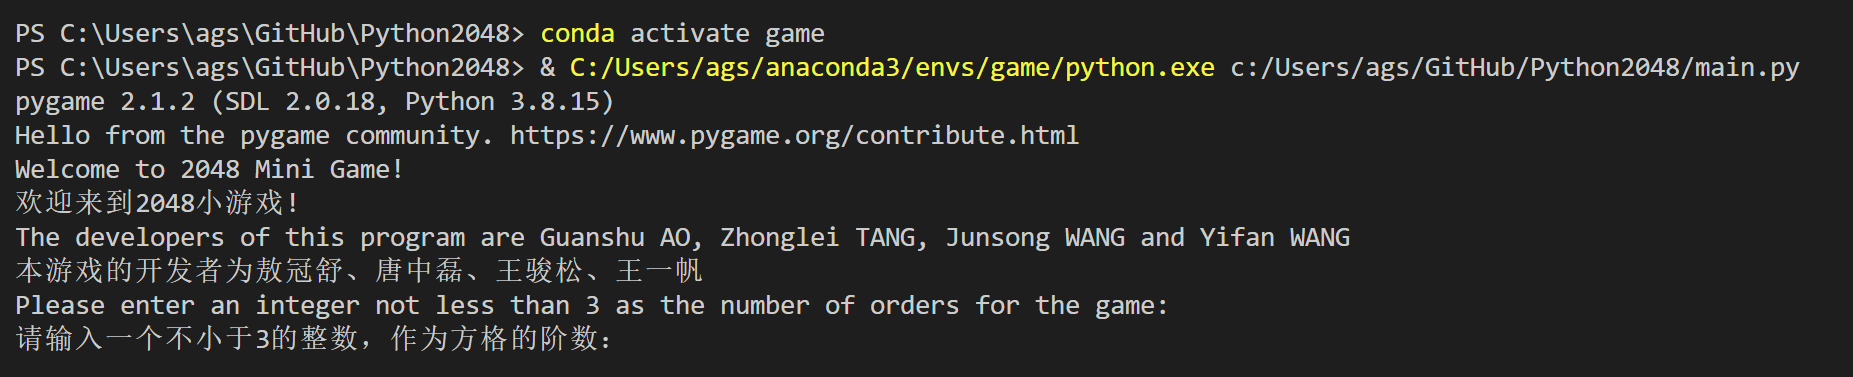
\includegraphics[width=0.7\linewidth]{img/pic1.png}
      \caption{控制台显示的内容}
      \label{fig:mergesort}
    \end{figure}
  \item 键入一个整数并回车(此处以4为例),即可开始游戏。如下图所示:
    \begin{figure}[!ht]
      \centering
      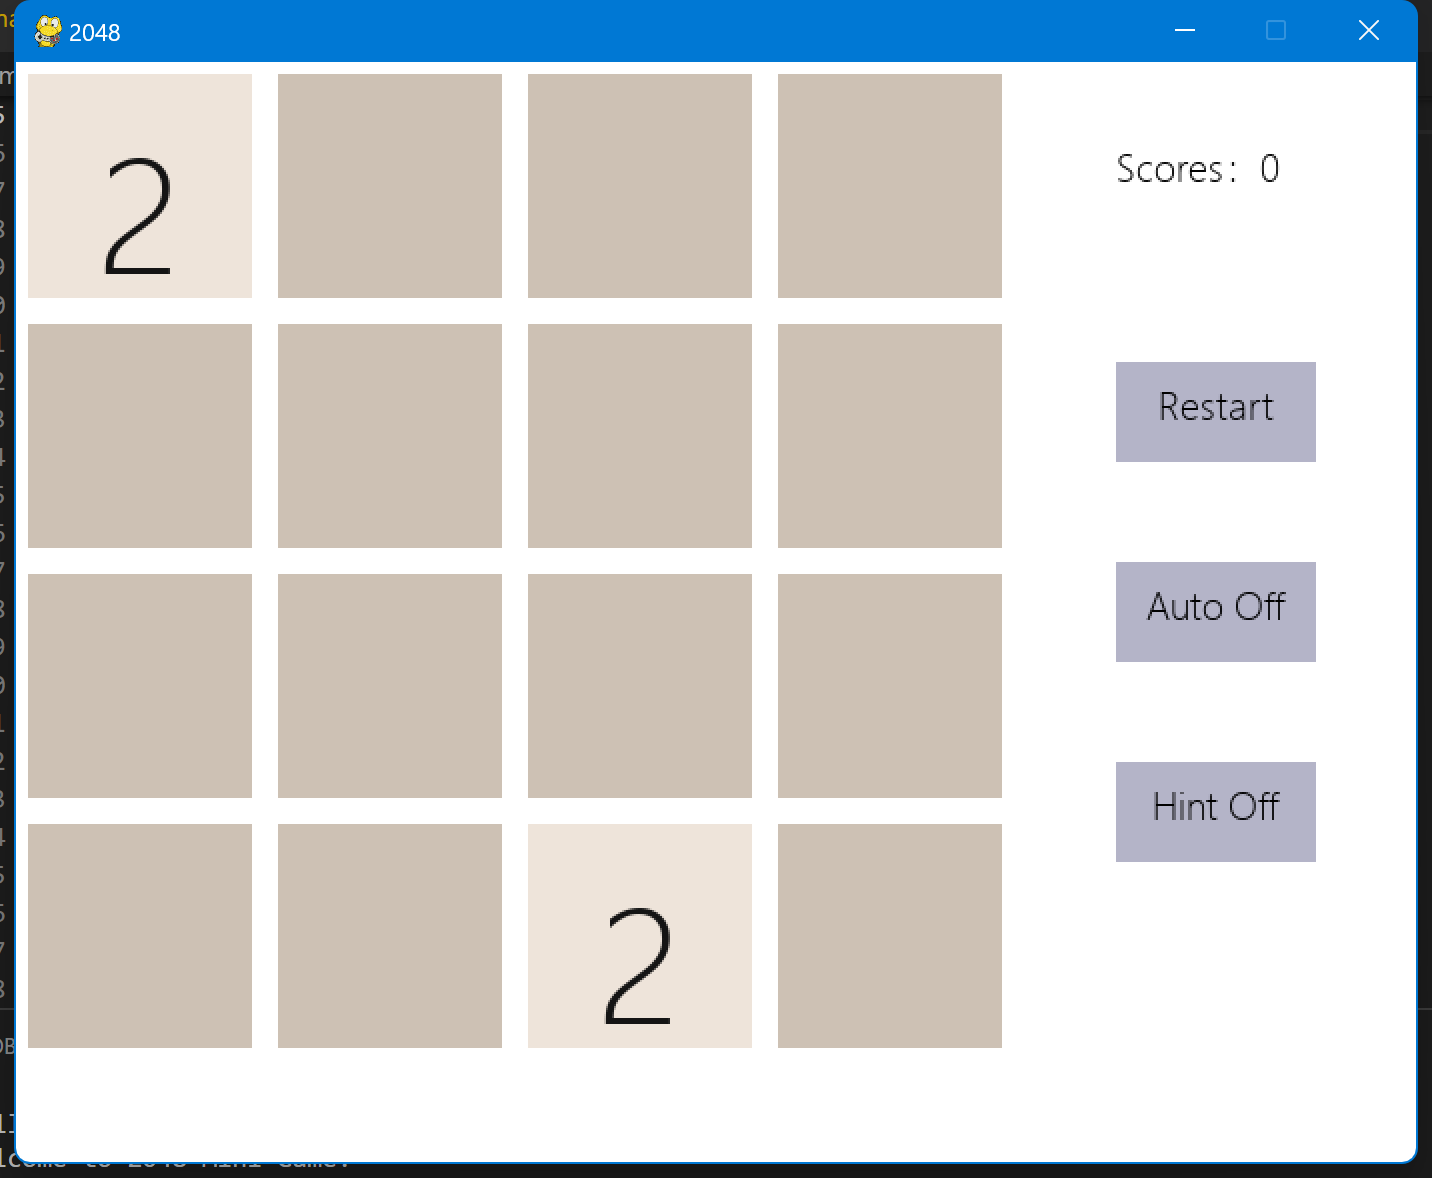
\includegraphics[width=0.7\linewidth]{img/pic2.png}
      \caption{四阶方格的2048游戏}
      \label{fig:mergesort}
    \end{figure}
  \item 此时可以通过键盘上的上下左右键来控制方块的移动,游戏界面的右上角会显示当前的得分。如下图所示:
    \begin{figure}[!ht]
      \centering
      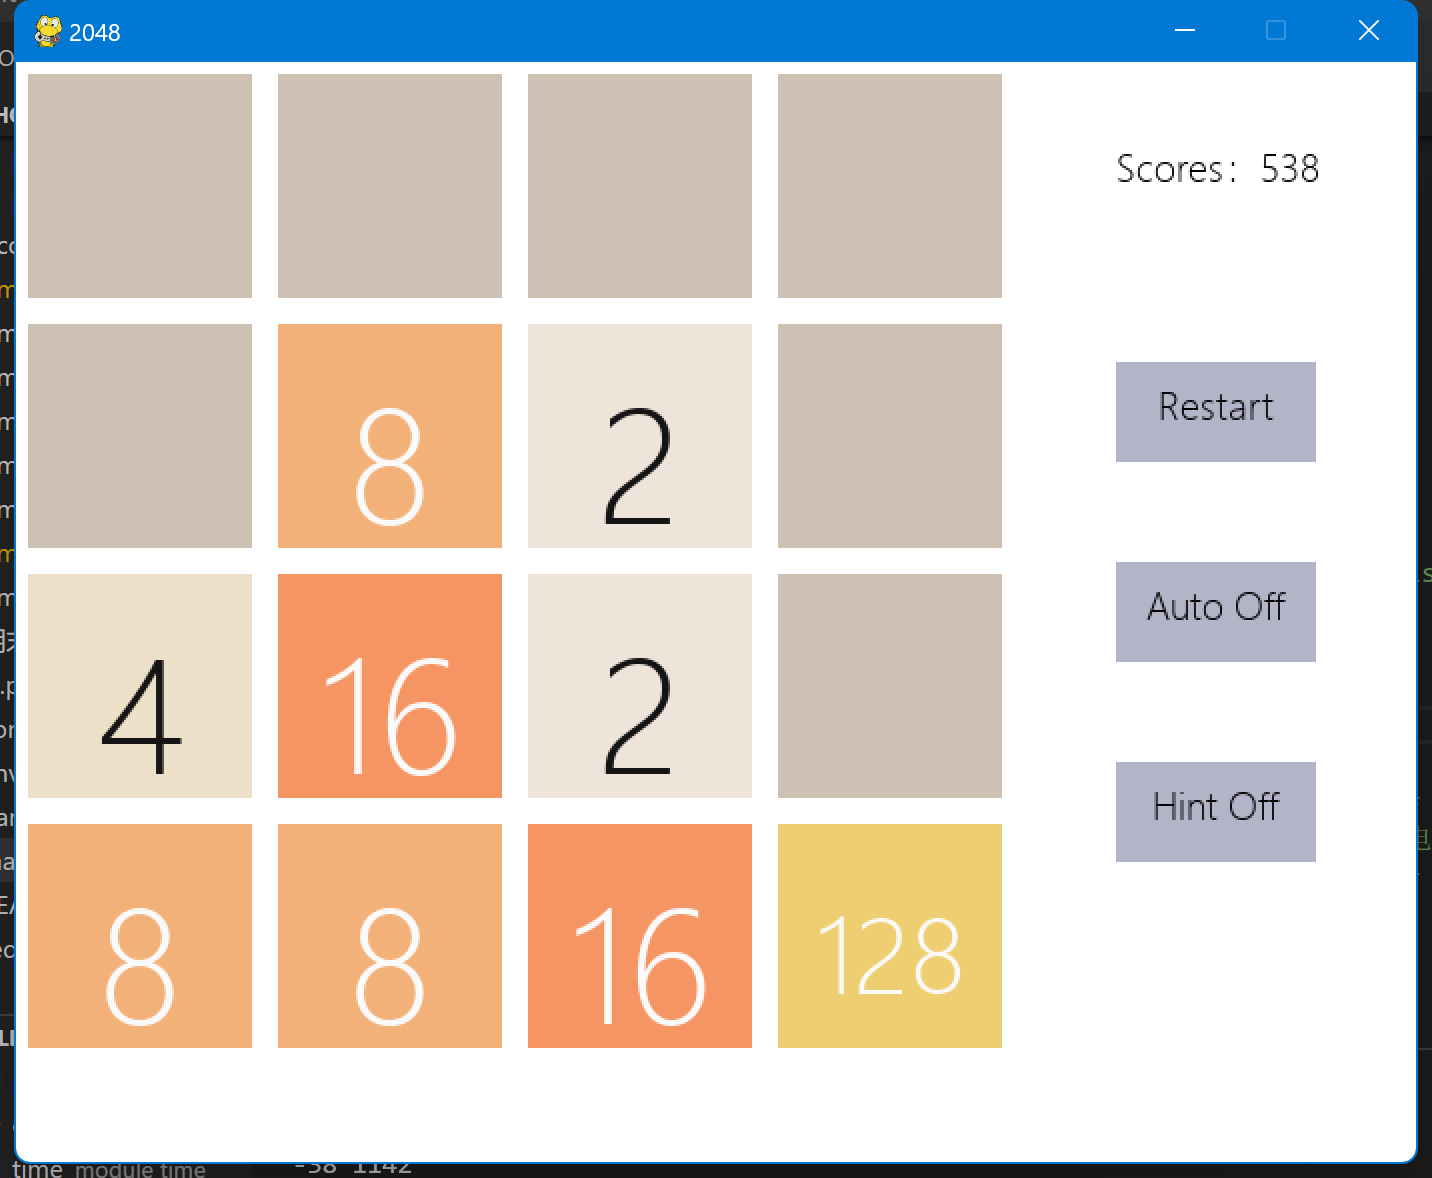
\includegraphics[width=0.7\linewidth]{img/pic3.png}
      \caption{正常模式}
      \label{fig:mergesort}
    \end{figure}
  \item 当游戏结束时,会显示游戏结束的提示,如下图所示:
    \begin{figure}[H]
      \centering
      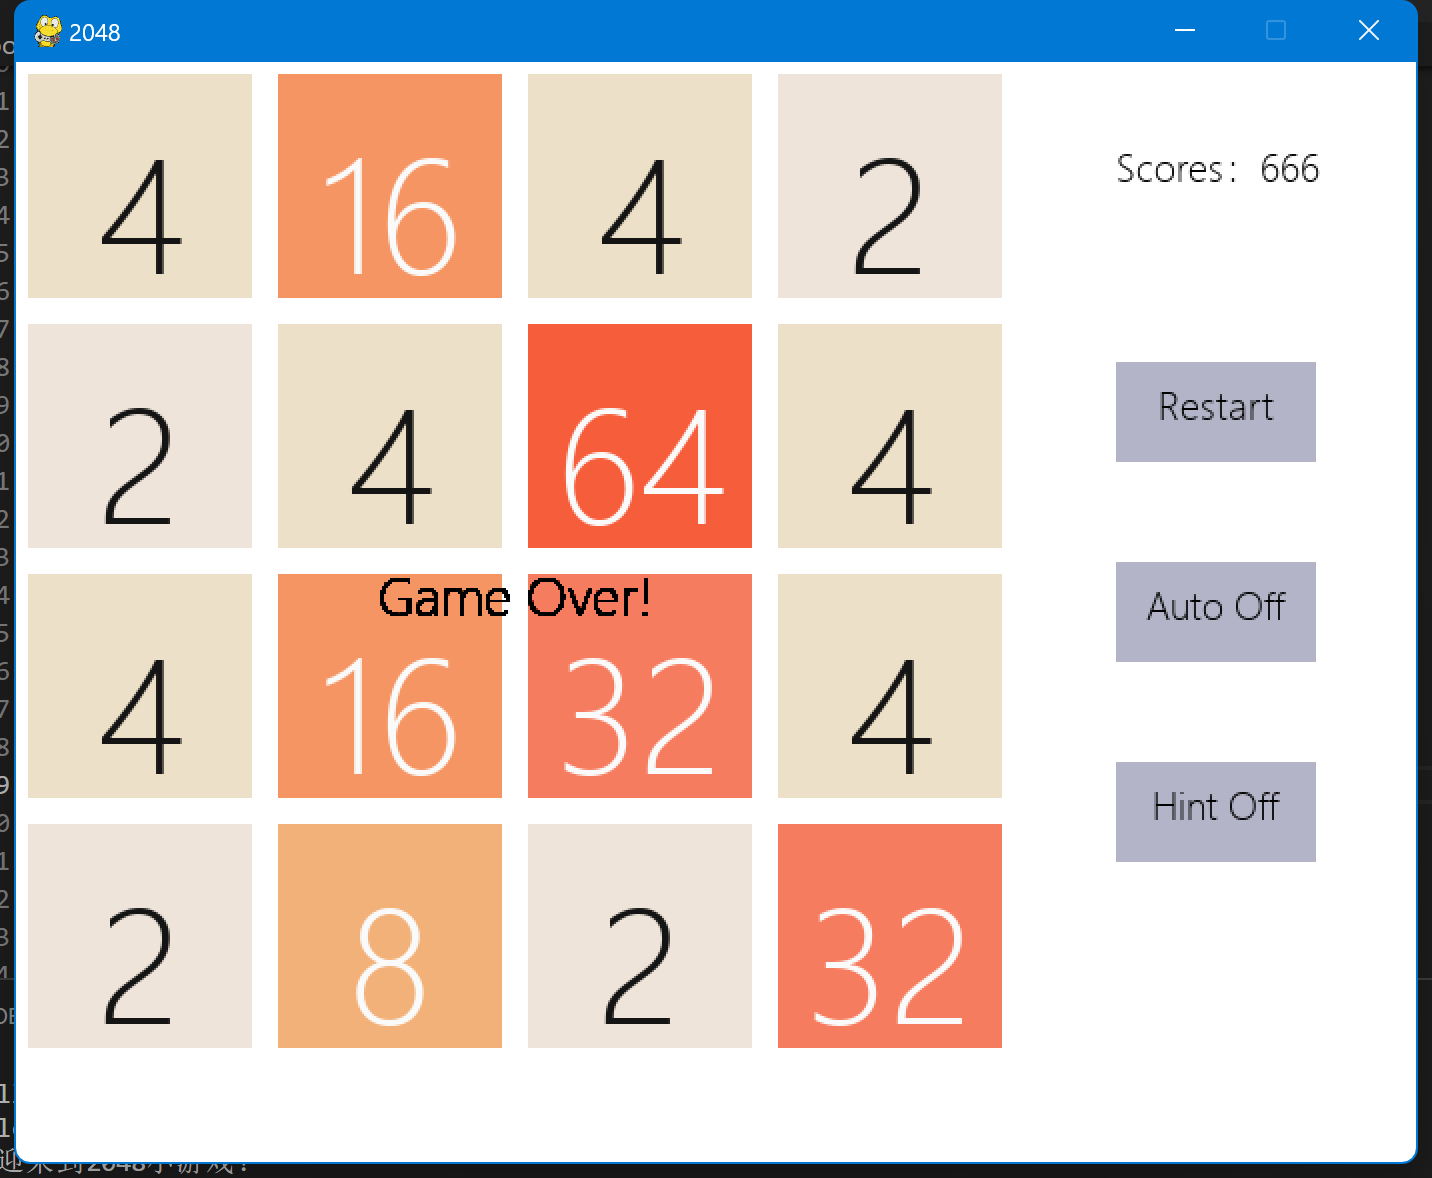
\includegraphics[width=0.7\linewidth]{img/pic4.png}
      \caption{游戏结束}
      \label{fig:mergesort}
    \end{figure}
  \item 在游戏过程中,点击Restart按钮,即可清空现有游戏进度重新开始。如下图所示:
    \begin{figure}[H]
      \centering
      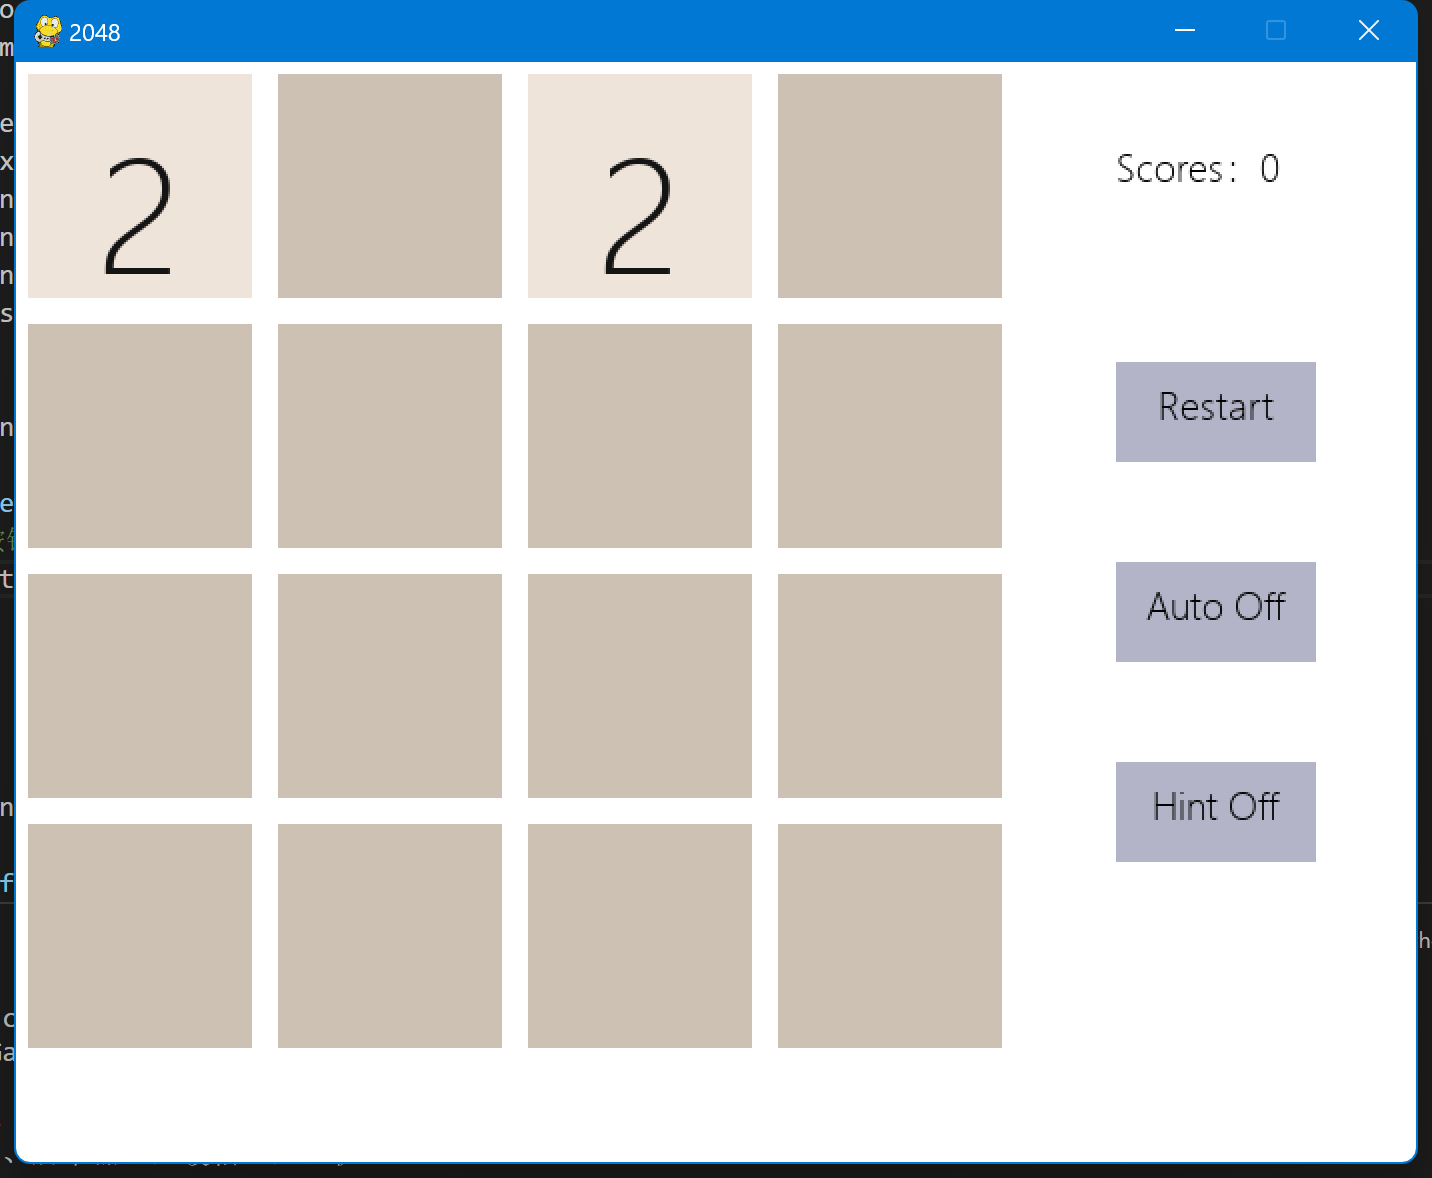
\includegraphics[width=0.6\linewidth]{img/pic5.png}
      \caption{重新开始游戏}
      \label{fig:mergesort}
    \end{figure}
  \item 右侧第二个按钮上显示Auto Off,表示现在处于手动模式。点击该按钮,即可切换到自动模式,在自动模式下,程序会自动寻找最优解并显示Auto On。再次点击按钮,即可恢复手动模式。具体情形如下图所示:
    \begin{figure}[H]
      \centering
      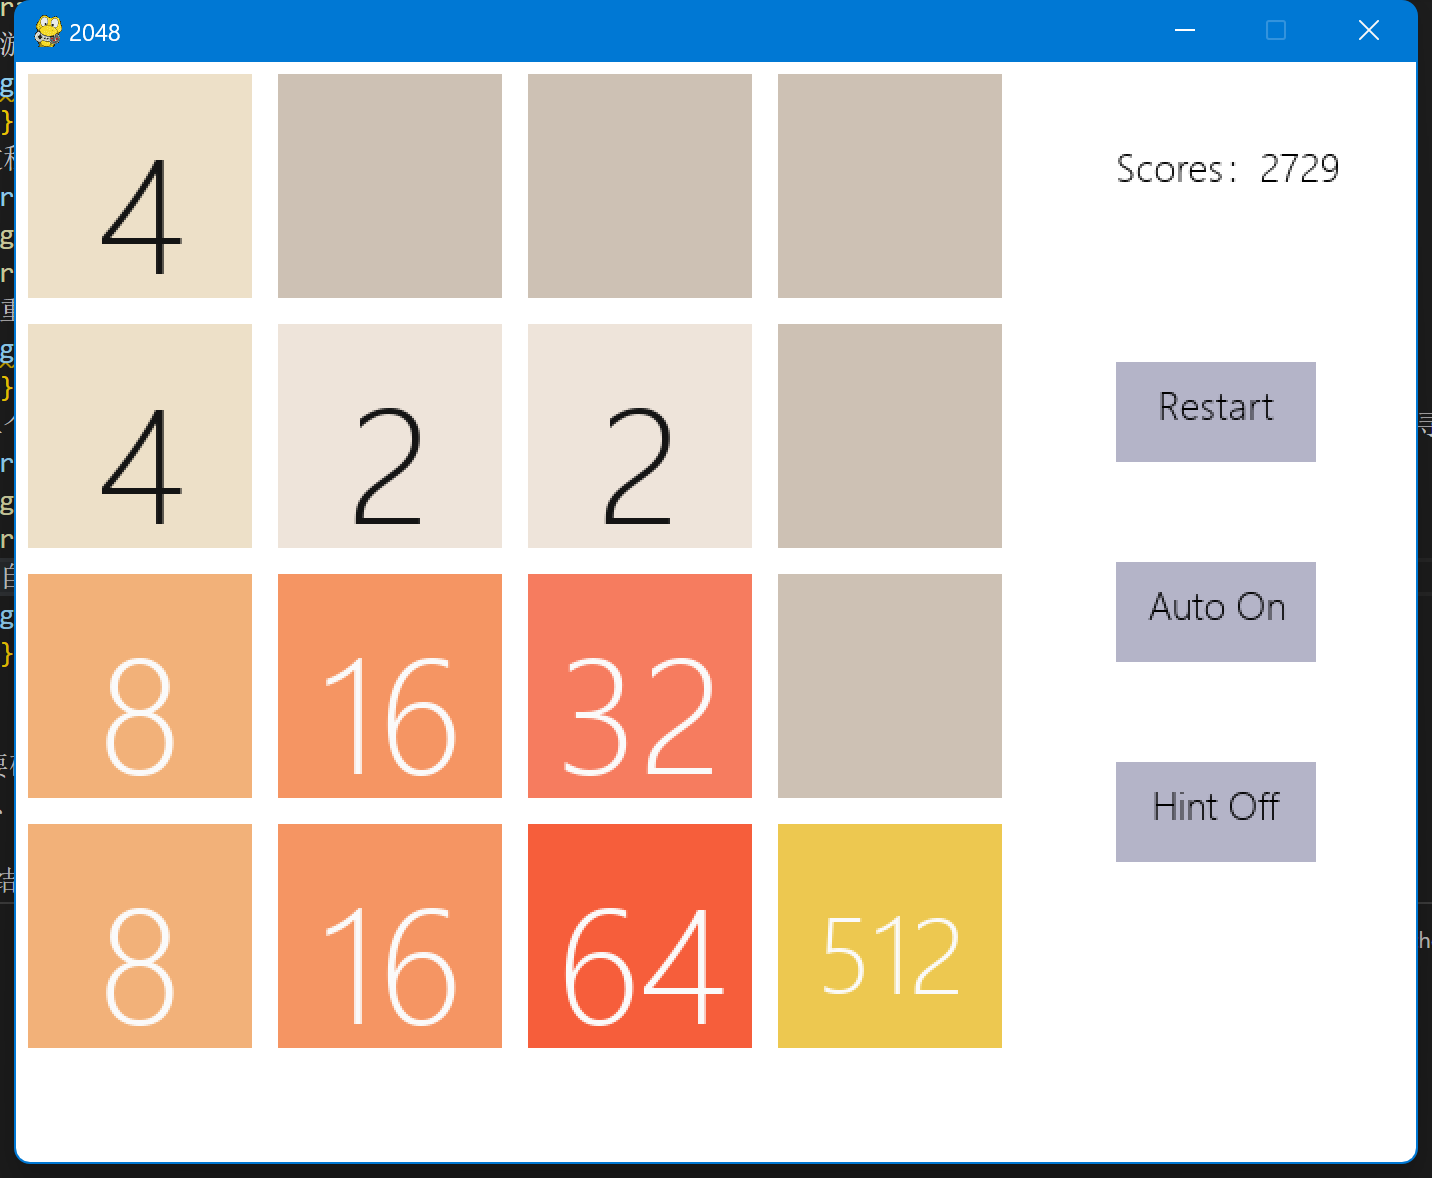
\includegraphics[width=0.6\linewidth]{img/pic6.png}
      \caption{自动模式}
      \label{fig:mergesort}
    \end{figure}
  \item 右侧第三个按钮显示Hint Off,表示现在未处于提示模式。点击该按钮即可切换到提示模式,在提示模式下,程序会显示当前最优解的方向,但不会自动操作。再次点击按钮,即可关闭提示模式。具体情形如下图所示:
    \begin{figure}[H]
      \centering
      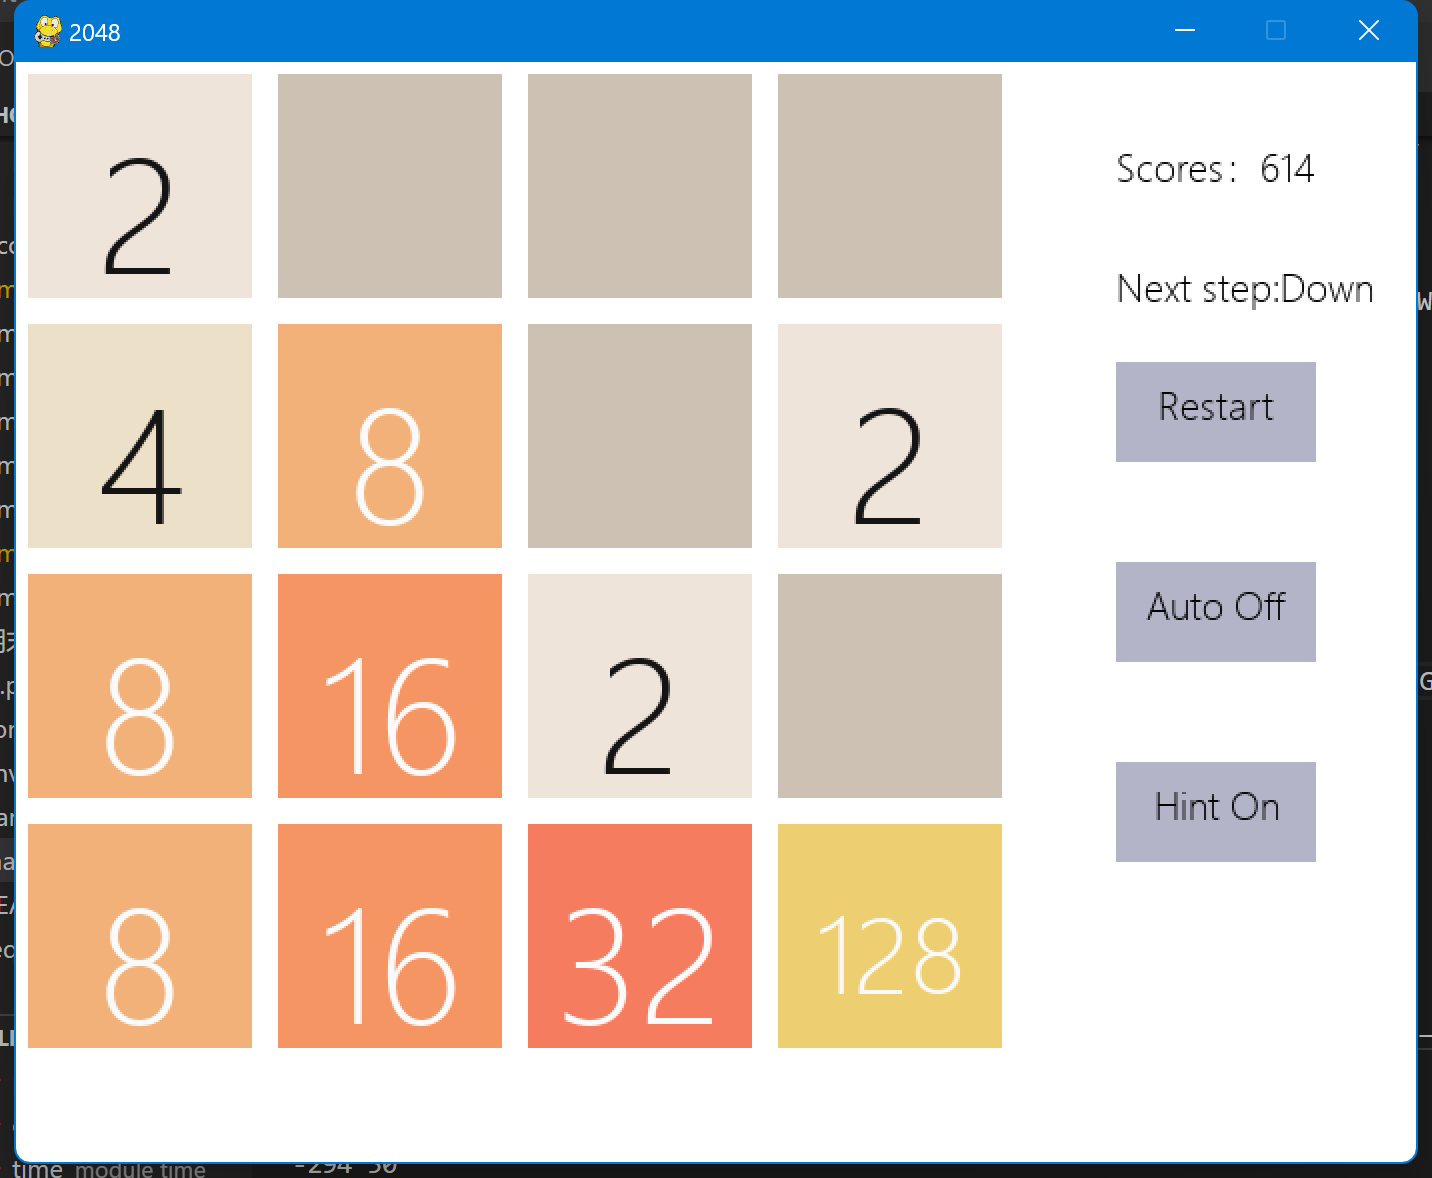
\includegraphics[width=0.5\linewidth]{img/pic7.png}
      \caption{提示模式}
      \label{fig:mergesort}
    \end{figure}
\end{itemize}

\subsection{特色功能}
相较于其他传统2048游戏,本程序新增了高阶方格下的游戏模式。只需在游戏开始时在终端输入想要的阶数,即可开始游戏。如下图所示,分别为6阶、10阶、20阶、40阶。其余功能与4阶方格下的游戏模式相同,不再赘述。
\begin{figure}[H]
  \centering
  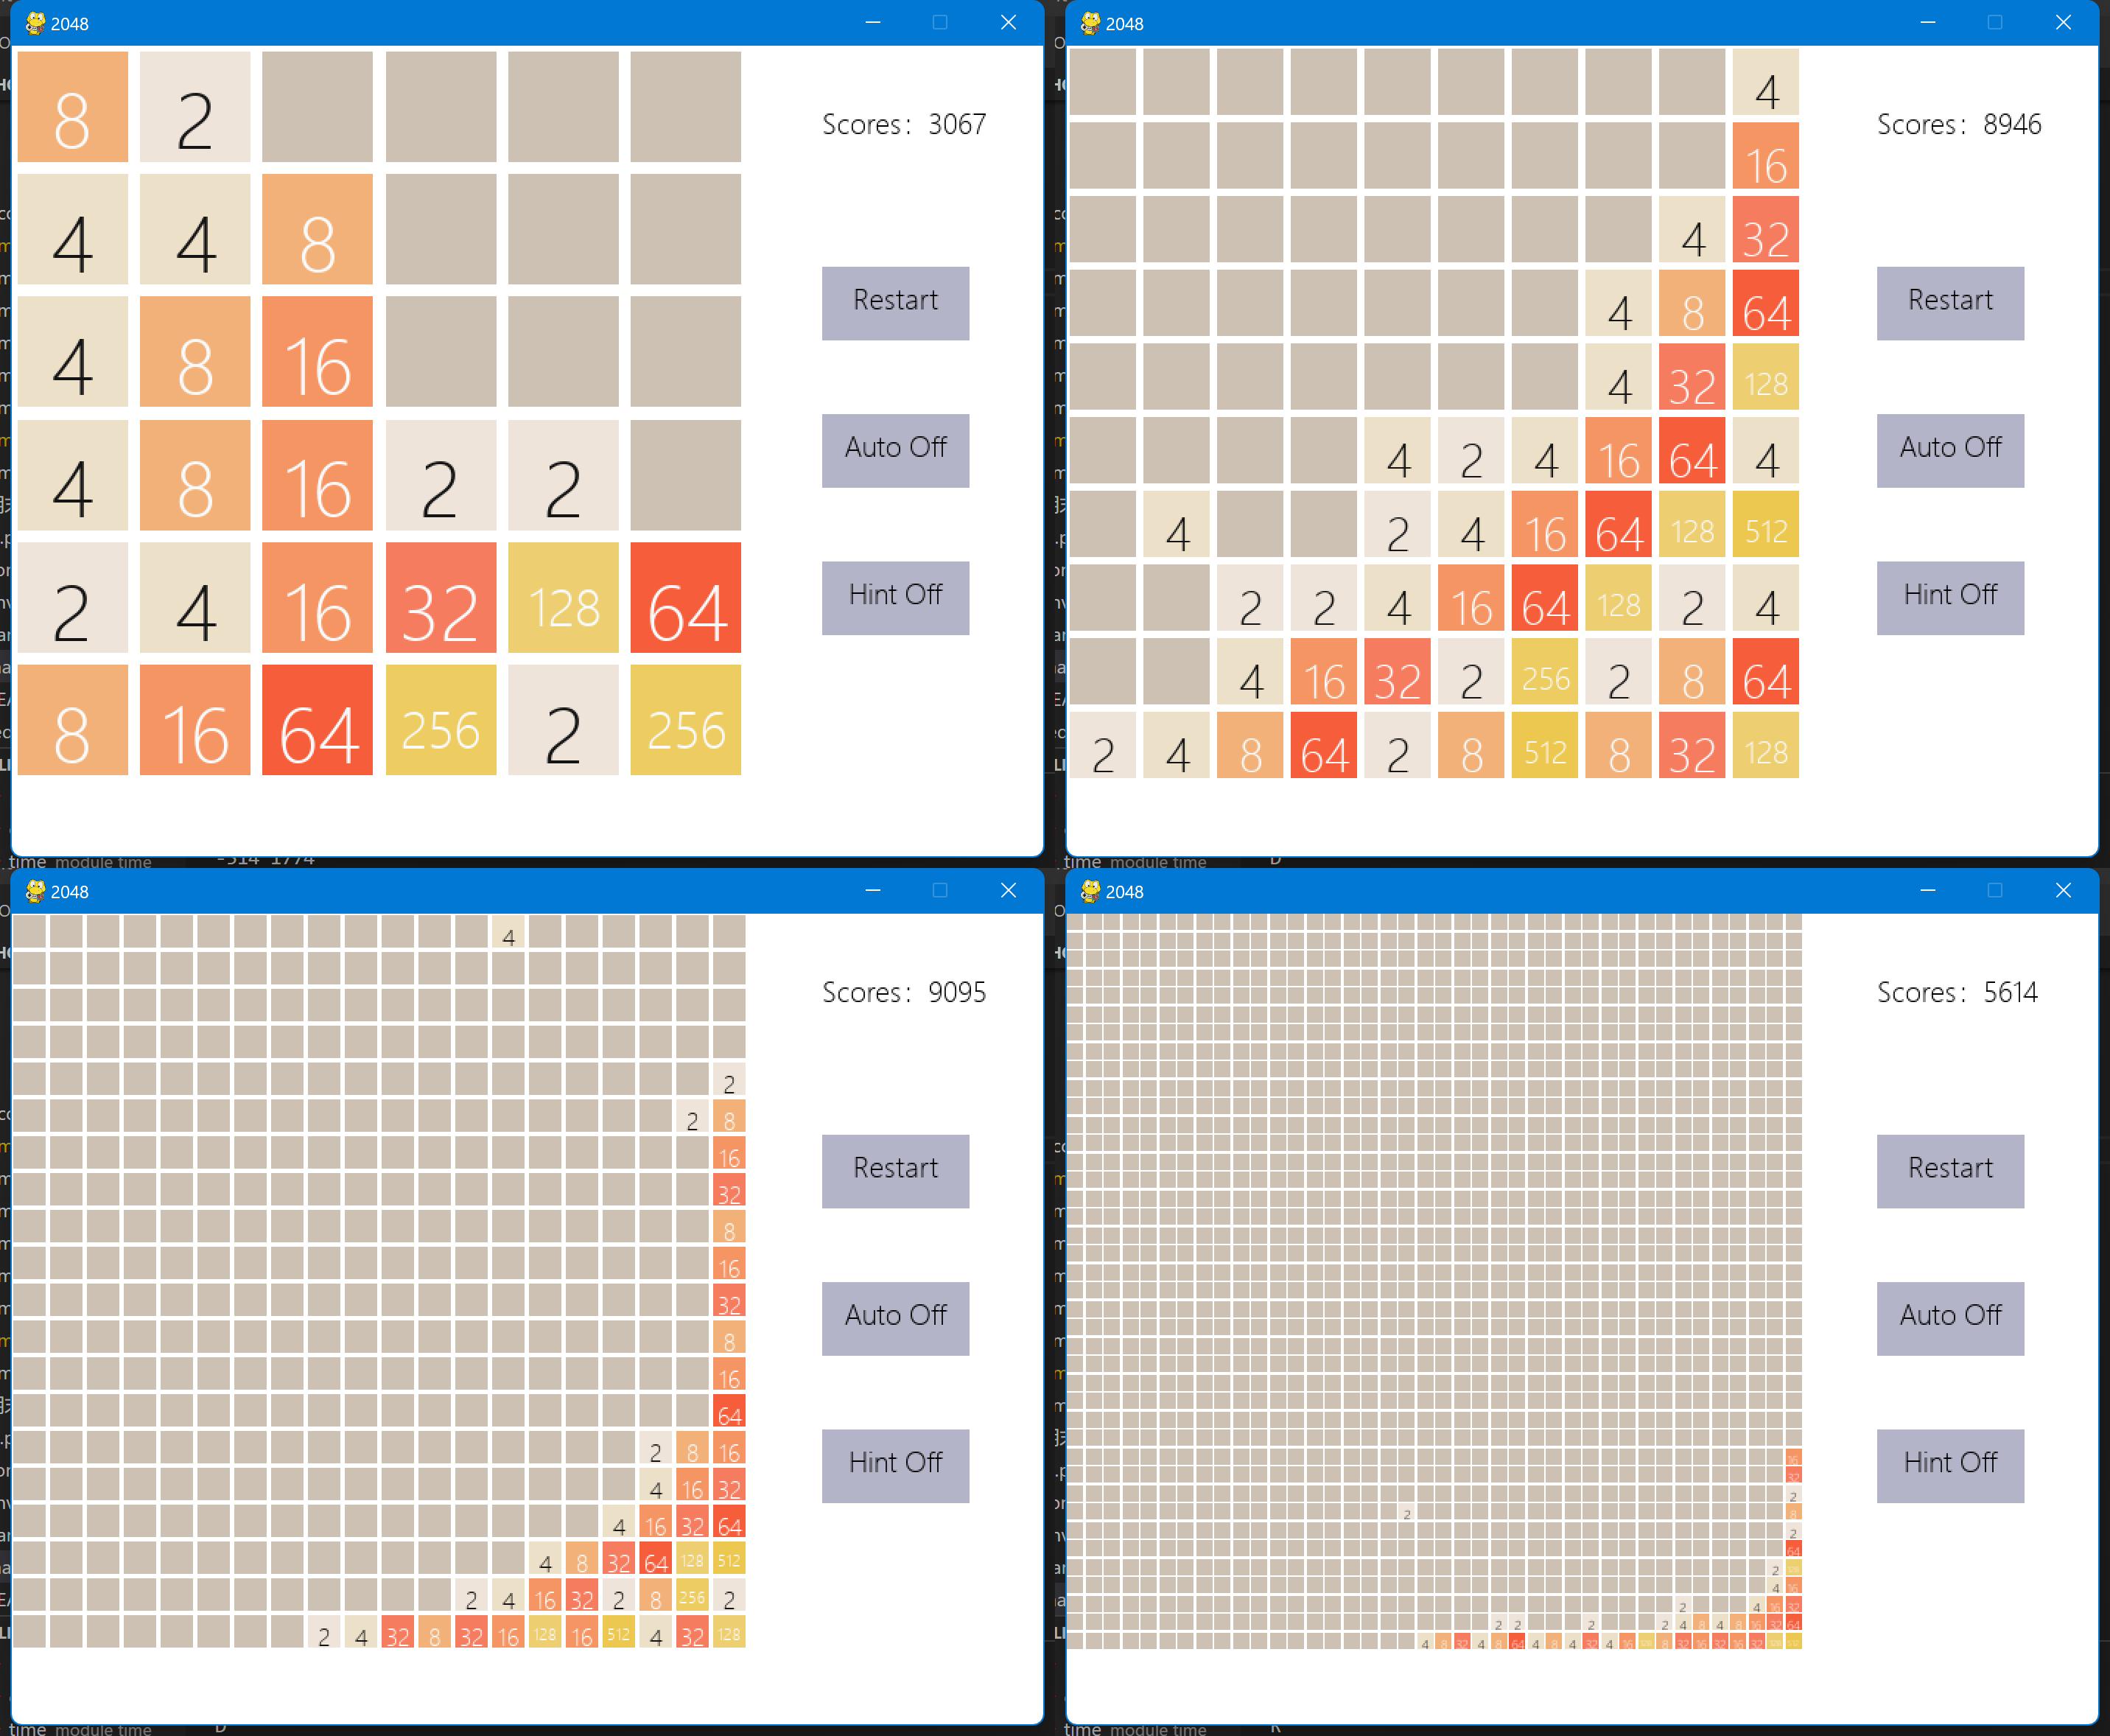
\includegraphics[width=0.55\linewidth]{img/pic12.png}
  \caption{高阶方格下的游戏模式}
  \label{fig:mergesort}
\end{figure}


\subsection{主要研究过程}
\begin{itemize}
  \item 首先,我们需要了解2048游戏的基本规则,即每次操作后,所有数字方块都会向一个方向移动,如果有两个相同的数字方块相邻,那么这两个数字方块会合并,合并后的数字方块的值为两个相加的和。如果有两个不同的数字方块相邻,那么这两个数字方块不会合并。如果有空白的位置,那么数字方块会移动到空白的位置。如果有两个数字方块相邻,中间有空白的位置,那么数字方块会移动到空白的位置。如果有两个数字方块中间有其他数字方块,那么这两个数字方块不会合并。
  \item 其次,我们需要了解2048游戏的算法。2048游戏的算法主要分为两个部分,一是生成新的数字方块,二是移动数字方块。
    \subitem 生成新的数字方块。在游戏开始时,会随机生成两个数字方块,每个数字方块的值为2或4。在游戏过程中,每次操作后,会随机生成一个数字方块,该数字方块的值为2或4。该数字方块会随机出现在空白的位置。
    \subitem 移动数字方块。从键盘读取用户的操作,根据键盘的操作,将数字方块向该方向移动,并生成新的状态矩阵。
  \item 最关键的是AI算法的实现。在本程序中,gen\_next首先会计算出一个数值 kn,它是当前棋盘的已有数字数量的平方与 20 之间的最小值,但是不能超过 40。然后使用 itertools 库的 product() 方法生成所有可能的移动序列,对于每个序列都调用 get\_grid() 方法和 get\_score() 方法来计算分数,并将结果存储在一个列表中。
  接着将所有序列的分数按照从小到大的顺序排序,然后从最高分的序列开始遍历,如果能够找到一个序列的第一个方向能够使得棋盘发生变化,就返回这个序列的第一个方向和平均分。如果所有序列都无法使棋盘发生变化,就返回最后一个序列的第一个方向和平均分。
  \item 在AI算法的基础上便可很容易地开发出提示功能。将AI算法的返回值改为提示的方向,显示在界面上即可实现提示功能。
\end{itemize}

\clearpage

\section{设计总结}

\subsection{成员分工}
四位成员均来自电子信息学院08062002班,其分工信息如下表所示:

\begin{table}[!ht]
  \centering
  \caption{成员分工一览表}
  \label{tab:progress}
  \begin{tabular}{@{}cllc@{}}
    \toprule
    姓名 & \multicolumn{1}{c}{学号} & \multicolumn{1}{c}{分工}    \\ \midrule
    敖冠舒 & 2020301928          & 总体方案设计、撰写报告、维护GitHub项目、AI算法实现、验收答辩     \\
    唐中磊 & 2020301923          & 游戏界面设计                   \\
    王骏松 & 2020301930          & 软件功能测试  \\ 
    王一帆 & 2020301927          & 方块移动模块的实现              \\ \bottomrule
  \end{tabular}
\end{table}

\subsection{当前程序不足之处}
总体来看,本程序的功能实现较为完整,较好地实现了指定的要求,并能在基本功能上进行扩展,如高阶方块模式,很好地增强了游戏的趣味性和丰富性。但由于时间和能力的限制,仍存在改进之处:

\begin{itemize}
  \item 可以将游戏开始时的方块阶数集成至游戏界面中而不是终端,方便用户选择
  \item 可以适当添加一些游戏音效和动效,增强游戏的趣味性
\end{itemize}

\subsection{改进措施}
对于以上存在的问题,小组成员计划采取以下措施进行改进:
\begin{itemize}
  \item 进一步学习用户界面设计,以期达到更好的用户体验
  \item 深入学习数据结构等相关知识,进一步优化当前算法,以期能够实现更加复杂的功能
\end{itemize}


\subsection{课程收获}
\begin{itemize}
  \item 敖冠舒
  \subitem 通过本课程的学习,我收获颇丰,受益匪浅。一方面精进了Python语言编程技能,对面向对象编程、模块化编程、数据结构、算法等方面的知识有了更深入的了解;另一方面,我也掌握了PyCharm、Anaconda、VSCode等开发工具的使用,利用GitHub进行团队协作,以及如何利用LaTeX进行文档编写等技能;此外,张老师邀请到的讲座嘉宾也令我大受启发。相信这些在今后的学习和工作中都会对我有所帮助,我也希望自己日后成为一名有技能、有格局的工程师,用技术造福更多的人,让每个人享受信息科技带来的便利!
  \item 唐中磊
  \subitem 在这学期课程学习中,我学习了Python的一些语言基础,很多知识与大一所学的C语言很相似,但也有很多不同,如Python的输入语句是print,而c语言的输入语句是printf,C语言一个语句的结束都要用分号隔开,而Python则不需要,又如在Python中定义变量是不需要先声明变量名及其类型的,而C语言则需要。而且,在字符串上的处理,Python相对于C语言更加简洁便利。除了这些基础语言知识,后边也学习了Python字典,库的使用,还有文件检索,以及函数的应用。在学习过程中,老师也会布置一些作业,也会组织一些考试,这对我们在Python学习的实际应用方面有所帮助,通过做这些作业和考试积累经验,逐步将Python的基础知识掌握。以及最后的大作业课程设计更好的帮助我们延申Python的学习,从小做起,慢慢熟练掌握Python完成更多更难的任务。因此学习Python不光要课堂上听老师讲课,课下的练习和实践更为重要,通过不断地学习和编程积累经验,更加深入的了解Python。
  \item 王骏松
  \subitem 初次学习Python,对于这学期的课程学习,学了Python的一些语言基础,很多知识与大一第一学期所学的c语言很相似,但有很多也是不同,如Python的输入语句是print,而c语言的输入语句是printf,c语言一个语句的结束都要用分号隔开,而Python则不需要,又如在Python中定义变量是不需要先声明变量名及其类型的,而c语言则需要。通过一学期的学习,我觉得Python比起C语言来说更为简洁简单,而c语言可以说是Python的基础。但Python虽然功能强大,操作起来也比较简单,但有一点是绝对不能忽视的,这是一门编程语言。学习Python之前一定要遵循一定的逻辑,不能急躁且盲目的乱学乱打编程,而是要循序渐进。作为一个初学者,在刚开始的学习中,我会按照课本中出现的代码,多进行实操,多打代码,多多学习别人的代码,希望能通过日积月累的学习不断提高我的编程能力,实现我一开始的学习目标。
  \item 王一帆
  \subitem Python是一种非常有潜力的高级语言,经过多年来的发展,已经在编程领域有了举足轻重的作用。经过一个学期的学习,我对Python有了一定的了解,明白了其强大的库对编程时起到的巨大作用,让编程不在困难。在学习Python的第一节课上,其对我的最初的印象就是,相较于我学习过的C语言编程,它更加的简洁。所有的变量都不需要像C语言编程那样需要提前去定义,这样给了编程者很大的自由空间与方便。对简化程序代码,起了很大作用。
\end{itemize}


\subsection{对课程的建议}
希望老师在日后的课程中能够更加注重实践,比如结合具体的程序和工程项目,这样让学生能够更加深刻的理解所学的知识,有助于学生更好地接触工程开发前沿。


\clearpage
\section{附录}
\subsection{程序源代码}

见电子压缩文档Python2048\_AGS.zip文件,或\href{https://github.com/guanshuao/Python2048/}{点击这里}查看本项目的GitHub仓库。

\subsection{其他}

\href{https://github.com/guanshuao}{作者的GitHub主页}

\href{https://guanshuao.github.io/}{作者的个人主页}

\href{https://github.com/guanshuao/Python2048/tree/main/Report}{本报告的LaTeX源码}

\subsection{致谢}

感谢张顺老师一学期以来的指导与帮助,您的严谨、亲和,以及专业的教学风格,让我在学习Python编程的过程中,不仅学到了知识,更学到了如何学习、如何思考,以及做学问的严谨态度。


\end{document}
